\documentclass{beamer}

\mode<presentation>
{
  \usetheme{AnnArbor} %Copenhagen
  \usecolortheme{wolverine}
  \setbeamercovered{transparent}
}

\usepackage[english]{babel}
\usepackage[latin1]{inputenc}
\usepackage{times}
\usepackage[T1]{fontenc} 
% Or whatever. Note that the encoding and the font should match. If T1
% does not look nice, try deleting the line with the fontenc.
\usepackage{amsmath}
\usepackage{graphicx}
\usepackage{multirow}

\newcommand{\linespace}{\vskip 0.25cm}

\definecolor{MyForestGreen}{rgb}{0,0.7,0} 
\newcommand{\tableemph}[1]{{#1}}
\newcommand{\tablewin}[1]{\tableemph{#1}}
\newcommand{\tablemid}[1]{\tableemph{#1}}
\newcommand{\tablelose}[1]{\tableemph{#1}}

\definecolor{MyLightGray}{rgb}{0.6,0.6,0.6}
\newcommand{\tabletie}[1]{\color{MyLightGray} {#1}}

% The text in square brackets is the short version of your title and will be used in the
% header/footer depending on your theme.
\title[Story of Rats]{Story of Rats:\\
					  An Examination of Co-Evolutionary Possibilities Between Rats and Humans}

% Sub-titles are optional - uncomment and edit the next line if you want one.
% \subtitle{Why does sub-tree crossover work?} 

% The text in square brackets is the short version of your name(s) and will be used in the
% header/footer depending on your theme.
\author[Dramdahl]{M. Kirbie Dramdahl}

% The text in square brackets is the short version of your institution and will be used in the
% header/footer depending on your theme.
\institute[U of Minn, Morris]
{
  University of Minnesota, Morris \\
  Morris, Minnesota, USA
}

% The text in square brackets is the short version of the date if you need that.
\date[Dec '14, Honors, UMM] % (optional)
{12 December 2014 \\ Honors Capstone Project Defense \\ University of Minnesota, Morris}

% Delete this, if you do not want the table of contents to pop up at
% the beginning of each subsection:
\AtBeginSection[]
{
  \begin{frame}<beamer>
    \frametitle{Outline}
    \tableofcontents[currentsection, hideothersubsections]
  \end{frame}
}

\begin{document}

\begin{frame}
  \titlepage
\end{frame}

% For a 20-25 minute senior seminar talk you probably want something like:
% - Two or three major sections (other than the summary).
% - At *most* three subsections per section.
% - Talk about 30s to 2min per frame. So there should probably be between
%   15 and 30 frames, all told.

\section*{Overview}

\subsection*{Outline}

\begin{frame}
\frametitle{Why?}
\begin{columns}
\begin{column}{.4\textwidth}
\begin{itemize}
\item complex relationship
\item personal experience
\end{itemize}
\end{column}
\begin{column}{.6\textwidth}
\begin{center}

\includegraphics[width=1\textwidth,trim={0 .45in 0 .45in}]{BanksyRat}
\linebreak
{\tiny Banksy}
\end{center}
\end{column}
\end{columns}
\end{frame}

\begin{frame}
  \frametitle{Outline}
  \tableofcontents[hideallsubsections]
\end{frame}

\section[Definitions]{Definitions}

\subsection[Rat and Human]{Rat and Human}

\begin{frame}
\frametitle{Definitions: Rat and Human}
\begin{center}
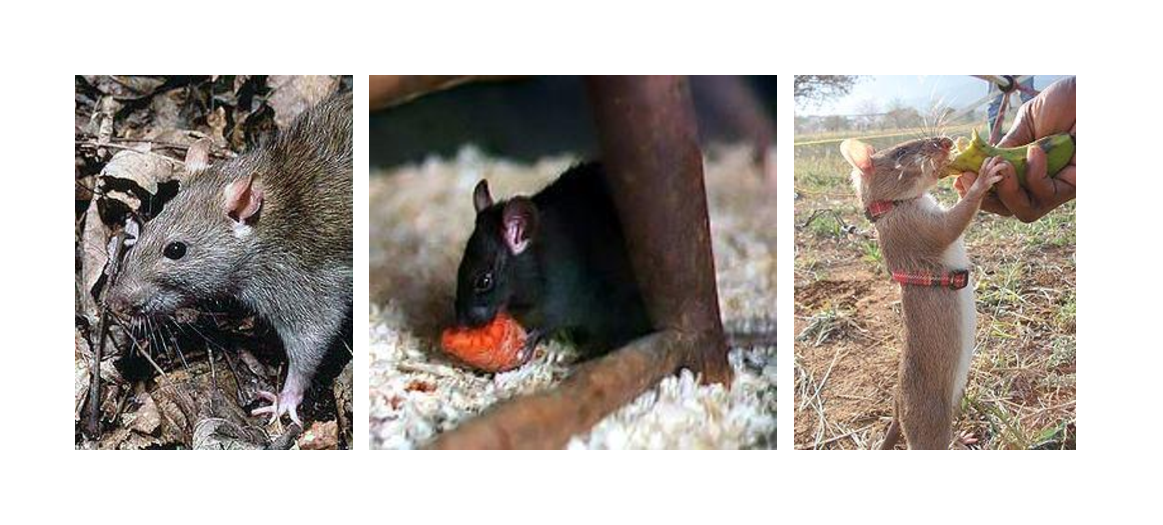
\includegraphics[width=1\textwidth,trim={0 .45in 0 .45in}]{RatVariations}
\linebreak
{\tiny Wikipedia}
\end{center}
\end{frame}

\subsection[Co-Evolution]{Co-Evolution}

\begin{frame}
\frametitle{Definitions: Co-Evolution}
\begin{columns}
\begin{column}{.5\textwidth}
Interactions
\begin{enumerate}
\item Competition
\item Mutualism
\item ``Enemy/Victim'' Interactions
\end{enumerate}
\end{column}
\begin{column}{.5\textwidth}
Processes
\begin{enumerate}
\item Patterns of Correlated Evolution (Phylogenetic Congruence)
\item Reciprocal Adaptive Responses
\begin{enumerate}
\item Specific Co-Evolution
\item Diffuse Co-Evolution
\end{enumerate}
\item Co-Speciation
\item Escape-and-Radiate Co-Evolution
\end{enumerate}
\end{column}
\end{columns}
\end{frame}

\subsection[Adaptation]{Adaptation}

\begin{frame}
\frametitle{Definitions: Adaptation}
Trait that confers enhanced reproductive success to an individual...
\begin{enumerate}
\item in the present,
\item not only in the present, but also in the past, and as a result is the product of natural selection, or
\item in the past, but which may or may not in the present, and may actually be maladaptive in the present.
\end{enumerate}
\end{frame}

\section[Topics]{Topics}

\subsection[Taxonomy]{Taxonomy}

\begin{frame}
\frametitle{Topics: Taxonomy}
\begin{center}
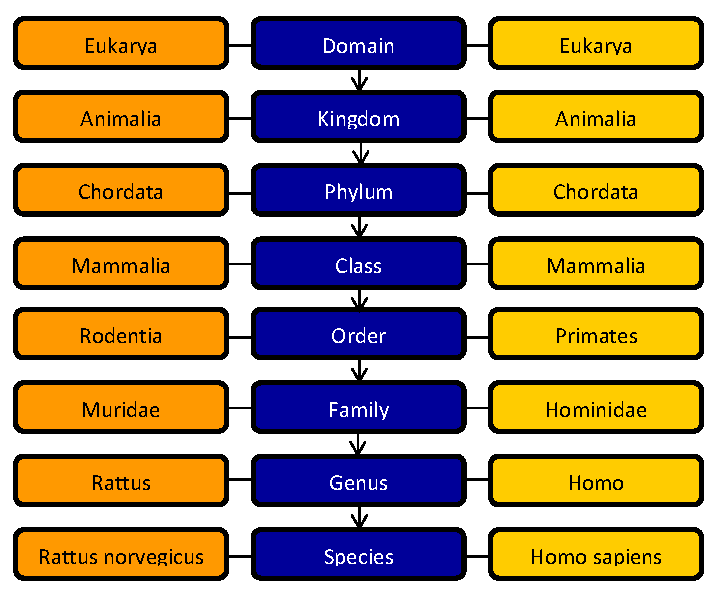
\includegraphics[width=.7\textwidth]{TaxonomyChart}
\end{center}
\end{frame}

\subsection[History]{History}

\begin{frame}
\frametitle{Topics: History}
\begin{columns}
\begin{column}{.3\textwidth}
Religion
\begin{itemize}
\item India
\item France
\item Israel
\linebreak
\end{itemize}
Literature
\begin{itemize}
\item Greece
\item England
\item United States
\end{itemize}
\end{column}
\begin{column}{.7\textwidth}
\begin{center}
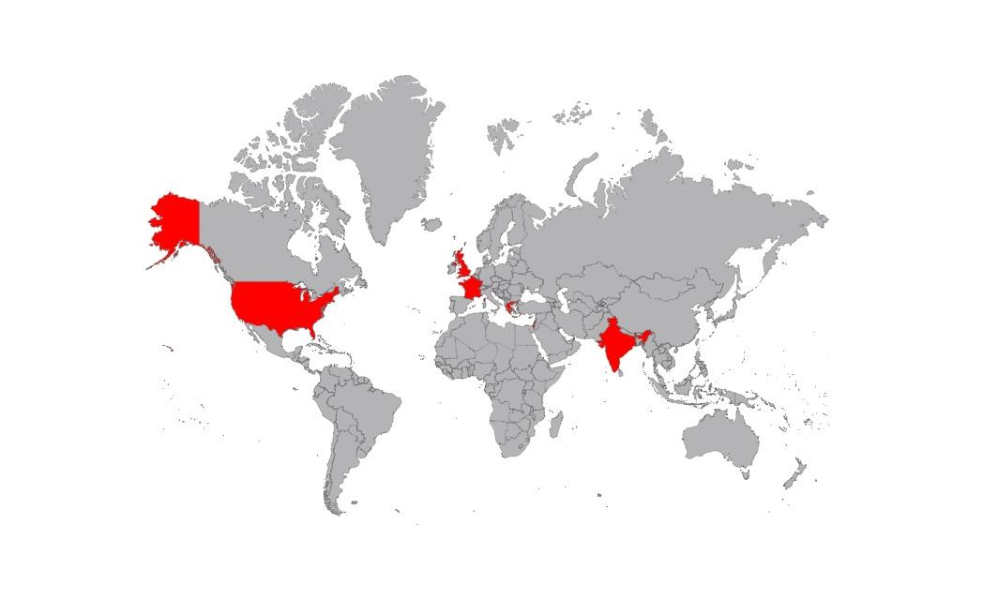
\includegraphics[width=1\textwidth,trim={0 .45in 0 .45in}]{WorldMap}
\linebreak
{\tiny amCharts}
\end{center}
\end{column}
\end{columns}
\end{frame}

\subsection[Current Cultural Identities of the Rat]{Current Cultural Identities of the Rat}

\begin{frame}
\frametitle{Topics: Current Cultural Identities of the Rat}
\begin{columns}
\begin{column}{.5\textwidth}
\begin{enumerate}
\item Vermin
\item Laboratory Animal
\item Pet
\end{enumerate}
\end{column}
\begin{column}{.5\textwidth}
\begin{center}
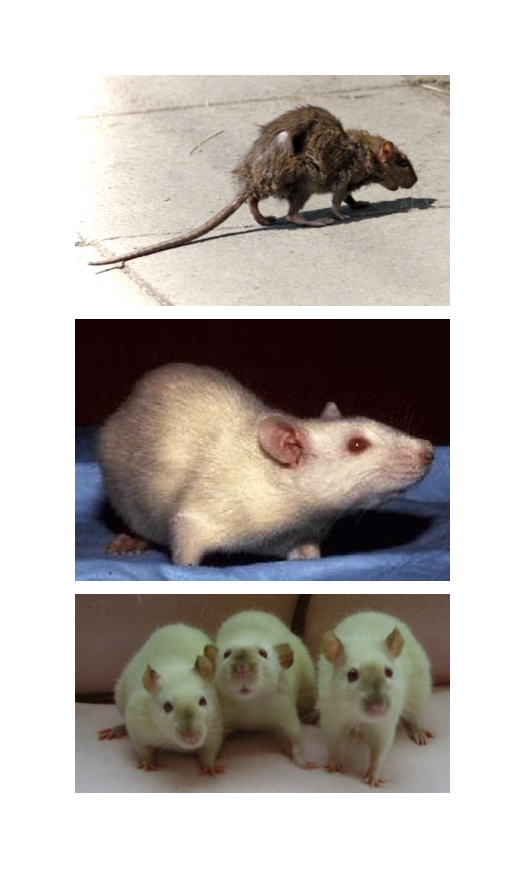
\includegraphics[width=.75\textwidth,trim={0 .45in 0 .45in}]{RatIdentities}
\linebreak
{\tiny Wikipedia}
\end{center}
\end{column}
\end{columns}
\end{frame}

\subsection[Case Study]{Case Study}

\begin{frame}
\frametitle{Topics: Case Study}
\begin{center}

\includegraphics[width=.5\textwidth,trim={0 .45in 0 .45in}]{APOPOLogo}
\linebreak
{\tiny APOPO}
\linebreak
\linebreak
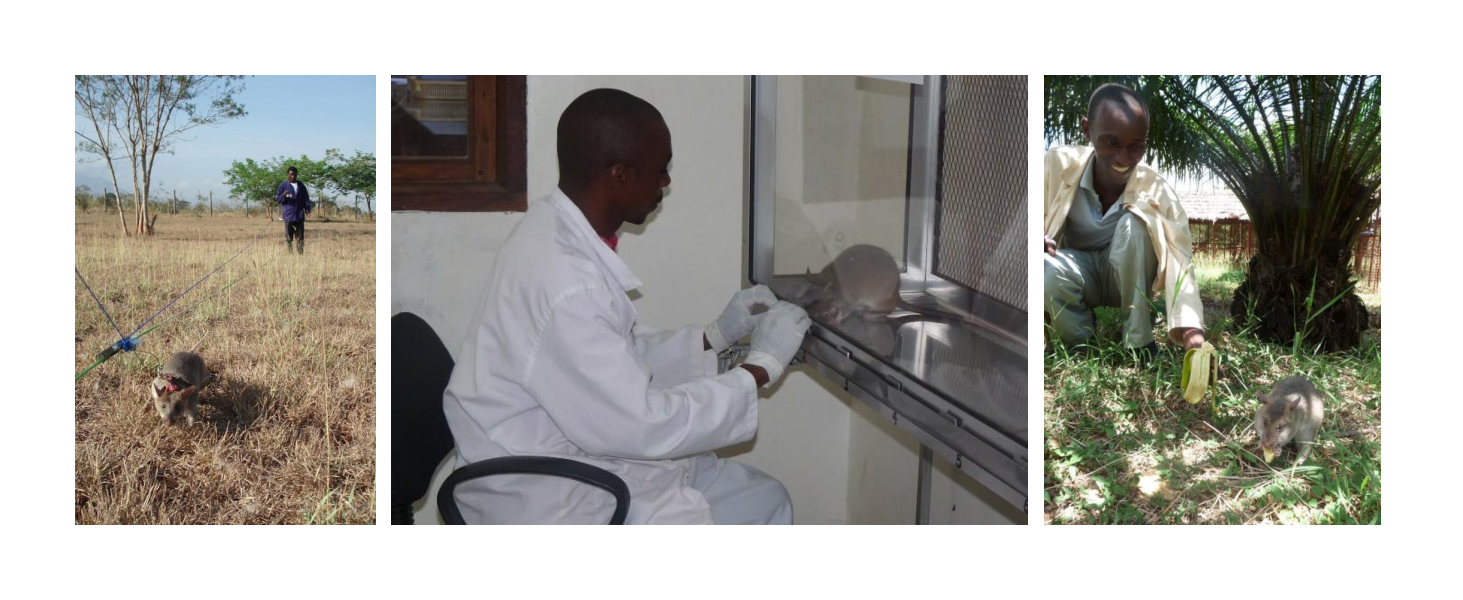
\includegraphics[width=.9\textwidth,trim={0 .45in 0 .45in}]{APOPOTraining}
\linebreak
{\tiny Wikipedia}
\end{center}
\end{frame}

\section[Conclusions]{Conclusions}

\begin{frame}
\frametitle{Conclusions}
\begin{columns}
\begin{column}{.5\textwidth}
Rats are highly adaptable...
\begin{itemize}
\item resources
\item distribution
\end{itemize}
\end{column}
\begin{column}{.5\textwidth}
Humans are highly adaptable...
\begin{itemize}
\item culture
\item technology
\end{itemize}
\end{column}
\end{columns}
\begin{center}
\end{center}
Some of these adaptations may or may not have happened in direct response to one another.
\end{frame}

\begin{frame}
\frametitle{Thanks!}
\begin{center}
Contact: \\ \texttt{dramd002@morris.umn.edu}
\linebreak
\linebreak
\linebreak
{\huge Questions?}
\end{center}
\end{frame}

%\section*{References}

%\begin{frame}[allowframebreaks] 
%\frametitle{References} 
%\nocite{*}
%\bibliographystyle{abbrv}
%{\tiny \bibliography{StoryOfRatsBibliography}}
%\end{frame}

\end{document}